\documentclass[slidestop,compress,mathserif]{beamer}
\usepackage{fontspec,xunicode,xltxtra,beamerthemesplit}
\usepackage{graphicx}
\usepackage{color}
\usepackage{xcolor}
\usepackage{multicol}
\usepackage{animate}
\usepackage[labelsep=quad]{caption}[2011/11/10]
\usepackage{float}
\usepackage{picins}

\renewcommand{\figurename}{}

\graphicspath{{figures/}}

%以下是各种演示主题,定义幻灯片中的所有细节
%\usetheme{default}
%\usetheme{Berlin}%这个主题比较好
%\usetheme{Pittsburgh}
%\usetheme{Rochester}
\usetheme{Berkeley}%这种演示主题比较好
%\usetheme{Goettingen}
%\usetheme{Hannover}
%\usetheme{Marburg}
%\usetheme{PaloAlto}%这种演示主题比较好
%\usetheme{Antibes}
%\usetheme{Darmstadt}
%\usetheme{JuanLesPins}
%\usetheme{Montpellier}
%\usetheme{Singapore}
%\usetheme{Boadilla}
%\usetheme{Madrid}
%\usetheme{AnnArbor}
%\usetheme{CambridgeUS}
%\usetheme{Copenhagen}
%\usetheme{Warsaw}

%以下是各种外部主题,确定幻灯的显示式样
%\useoutertheme{infolines}
%\useoutertheme{miniframes}
%\useoutertheme[height=0.1\textwidth,width=0.15\textwidth,hideothersubsections]{sidebar}
%\useoutertheme{smoothbars}
%\useoutertheme{split}
%\useoutertheme{shadow}
%\useoutertheme{tree}
%\useoutertheme{smoothtree}
%\useoutertheme[height=0.5\textwidth]{sidebar}

%以下是各种内部主题
%\useinnertheme{default}
%\useinnertheme{circles}
%\useinnertheme{rectangles}
\useinnertheme[shadow]{rounded}

%以下是各种颜色主题
%\usecolortheme{default}
%\usecolortheme{albatross}
%\usecolortheme{beaver}
%\usecolortheme{beetle}
%\usecolortheme{crane}
%\usecolortheme{dolphin}
%\usecolortheme{dove}
%\usecolortheme{fly}
%\usecolortheme{lily}
%\usecolortheme{orchid}
%\usecolortheme{rose}
%\usecolortheme{seagull}
\usecolortheme{seahorse}
%\usecolortheme{sidebartab}
%\usecolortheme{structure}
%\usecolortheme{whale}
%\usecolortheme{wolverine}

%以下是各种字体主题
%\usefonttheme{default}
%\usefonttheme[onlymath]{serif}
%\usefonttheme{structurebold}
%\usefonttheme{structureitalicserif}
%\usefonttheme{structuresmallcapsserif}

\setsansfont[Mapping=tex-text, BoldFont={Microsoft YaHei Bold}]{Microsoft YaHei}
%\setsansfont[Mapping=tex-text, BoldFont={Songti SC Bold}]{Songti SC}

% 中文环境自动换行
\XeTeXlinebreaklocale "zh"  % 表示用中文的断行
\XeTeXlinebreakskip = 0pt plus 1pt % 多一点调整的空间

% 中文环境修正导航栏
\makeatletter
\setbeamertemplate{blocks}[rounded][shadow=true] 
\def\beamer@linkspace#1{
  \begin{pgfpicture}{0pt}{-1.5pt}{#1}{5.5pt}
    \pgfsetfillopacity{0}
    \pgftext[x=0pt,y=-1.5pt]{.}
    \pgftext[x=#1,y=5.5pt]{.}
  \end{pgfpicture}}
\makeatother

% 超链接高亮显示
\hypersetup{CJKbookmarks=true,
colorlinks=true,
citecolor=blue,
linkcolor=blue,
urlcolor=blue,
bookmarksopen=true,
breaklinks=true
}


% 幻灯片切换方式
%\transblindshorizontal 	% 水平百叶窗
%\transblindsvertical 		% 垂直百叶窗
%\transboxin				% 盒状收缩
%\transboxout				% 盒状展开
%\transdissolve				% 溶解
%\transglitter
%\transsplithorizontalin	% 上下向中央收缩
%\transsplitverticalin		% 垂直向中央收缩
%\transsplithorizontalout	% 上下向中央展开
%\transsplitverticalout		% 垂直向中央展开
%\transwipe					% 从下抽出


\title{2002年图灵奖~\\~公钥密码学~\\~RSA加密算法}
\author{刘正~~徐小奇}
\date{\today}
%\institute{同济大学电信学院}

\logo{\color{blue!50}\scalebox{2}{{
\includegraphics[height=0.8cm]{logo.jpg}\vspace{220pt}}}}

% 设定frametitle居中
\makeatletter 
\long\def\beamer@@frametitle[#1]#2{% 
  \beamer@ifempty{#2}{}{% 
    \gdef\insertframetitle{\centering{#2\ifnum\beamer@autobreakcount>0\relax{}\space\usebeamertemplate*{frametitle continuation}\fi}}% 
  \gdef\beamer@frametitle{#2}% 
  \gdef\beamer@shortframetitle{#1}% 
}% 
} 
\makeatother


\begin{document}

\frame{\titlepage}

\section{RSA加密算法}

\begin{frame}
  \transdissolve
  \frametitle{加密的历史}
  
  \begin{block}<+->{1976年以前,所有的加密方法都是同一种模式:}
    \begin{itemize}[<+->]
        \item 甲方选择某一种加密规则,对信息进行加密;
        \item 乙方使用同一种规则,对信息进行解密。
    \end{itemize}
  \end{block}

\end{frame}

\begin{frame}
  \frametitle{加密的历史}
  
  \begin{block}{1976年以前,所有的加密方法都是同一种模式:}
    \begin{itemize}
        \item 甲方选择某一种加密规则,对信息进行加密;
        \item 乙方使用同一种规则,对信息进行解密。
    \end{itemize}
  \end{block}
  ~\\[0.6cm]

~ ~ ~ ~由于加密和解密使用同样规则(简称"密钥"),这被称为"对称加密算法"(Symmetric-key algorithm)。

~ ~ ~ ~这种加密模式有一个最大弱点:甲方必须把加密规则告诉乙方,否则无法解密。保存和传递密钥,就成了最头疼的问题。
\end{frame}

\subsection{\hfill 凯撒密码}
\begin{frame}
  \frametitle{凯撒密码}
\end{frame}
\begin{frame}
  \frametitle{凯撒密码}
  ~~~~字母之间的替换---它的几个变种:换字式密码(破解的方法可以使用字符频数分析法)、转置式密码、多表替换密码(先分组后凯撒加密)
\end{frame}
\begin{frame}
\transboxout
  \frametitle{凯撒密码}
  ~~~~字母之间的替换---它的几个变种:换字式密码(破解的方法可以使用字符频数分析法)、转置式密码、多表替换密码(先分组后凯撒加密)
  \begin{figure}
    \centering
    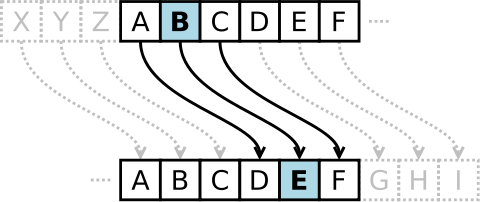
\includegraphics[width=5cm]{Caesar3.png}
  \end{figure}
\end{frame}


%\begin{frame}
%  \frametitle{凯撒密码}
%  \begin{itemize}[<+->]
%    \item{明文字母表:}ABCDEFGHIJKLMNOPQRSTUVWXYZ
%    \item{密文字母表:}DEFGHIJKLMNOPQRSTUVWXYZABC
%    \item{明文:}THE QUICK BROWN FOX JUMPS OVER THE LAZY DOG
%    \item{密文:}WKH TXLFN EURZQ IRA MXPSV RYHU WKH ODCB GRJ
%    \end{itemize}
%
%\end{frame}
%\begin{frame}
%  \frametitle{凯撒密码}
%  \begin{itemize}
%    \item{明文字母表:}ABCDEFGHIJKLMNOPQRSTUVWXYZ
%    \item{密文字母表:}DEFGHIJKLMNOPQRSTUVWXYZABC
%    \item{明文:}THE QUICK BROWN FOX JUMPS OVER THE LAZY DOG
%    \item{密文:}WKH TXLFN EURZQ IRA MXPSV RYHU WKH ODCB GRJ
%    \end{itemize}
%  恺撒密码的加密、解密方法还能够通过同余的数学方法进行计算。首先将字母用数字代替,A=0,B=1,\ldots,Z=25。此时偏移量为n的加密方法即为:
%
%  \begin{equation}
%    E_n=(x+n) ~mod~ 26
%  \end{equation}
%  解密就是:
%  \begin{equation}
%    D_n=(x-n) ~mod~ 26
%  \end{equation}
%
%\end{frame}


\subsection{\hfill 栅栏密码}
\begin{frame}
  \frametitle{栅栏密码}
\end{frame}
\begin{frame}
  \transwipe
  \frametitle{栅栏密码}
%加密的明文分成N个一组,然后把每组的第1个字连起来,形成一段无规律的话
  ~\\[1.6cm]
    ~~~~所谓栅栏密码,就是把要加密的明文分成N个一组,然后把每组的第1个字连起来,形成一段无规律的话。 不过栅栏密码本身有一个潜规则,就是组成栅栏的字母一般不会太多。(一般不超过30个,也就是一、两句话)
\end{frame}

%\subsection{\hfill 维基尼亚密码}
%\begin{frame}
%  \frametitle{维基尼亚密码}
%引入密钥 对抗字频统计既同一个密文字符对应该的明文不一定是相同的)
%\end{frame}
\subsection{\hfill RSA加密算法}
\begin{frame}
  \frametitle{RSA加密算法}
\end{frame}
\begin{frame}
  \transsplitverticalin
  \frametitle{RSA加密算法}
 ~ ~ ~ ~RSA加密算法是一种非对称加密算法。在公开密钥加密和电子商业中RSA被广泛使用。

~ ~ ~ ~ RSA是1977年由罗纳德·李维斯特(Ron Rivest)、阿迪·萨莫尔(Adi Shamir)和伦纳德·阿德曼(Leonard Adleman)一起提出的。当时他们三人都在麻省理工学院工作。RSA就是他们三人姓氏开头字母拼在一起组成的。

~ ~ ~ ~ 1973年,在英国政府通讯总部工作的数学家克利福德·柯克斯(Clifford Cocks)在一个内部文件中提出了一个相同的算法,但他的发现被列入机密,一直到1997年才被发表。

\end{frame}


\begin{frame}
  \transboxout
  \frametitle{RSA加密算法}
  \begin{center}
    \begin{figure}
      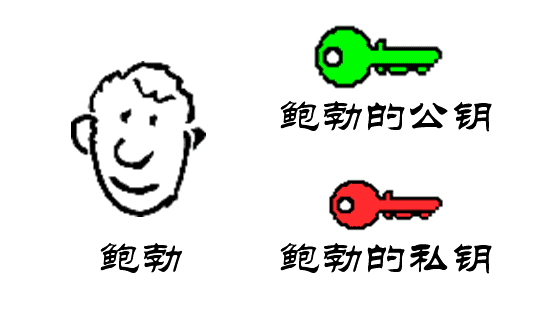
\includegraphics[width=8cm]{bg1}
    \end{figure}
    鲍勃有两把钥匙,一把是公钥,另一把是私钥。
  \end{center}
\end{frame}

\begin{frame}
  \transboxout
  \frametitle{RSA加密算法}
  \begin{center}
    \begin{figure}
      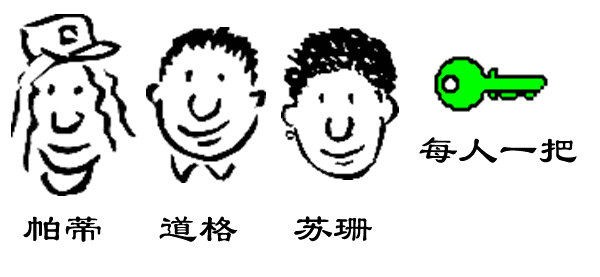
\includegraphics[width=8cm]{bg2}
    \end{figure}
  \end{center}
  鲍勃把公钥送给他的朋友们----帕蒂、道格、苏珊----每人一把。
\end{frame}

\begin{frame}
  \transboxout
  \frametitle{RSA加密算法}
  \begin{center}
    \begin{figure}
      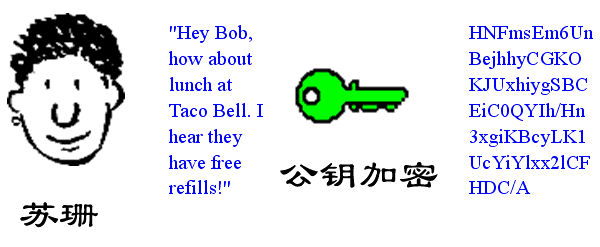
\includegraphics[width=8cm]{bg3}
    \end{figure}
    苏珊要给鲍勃写一封保密的信。她写完后用鲍勃的公钥加密,就可以达到保密的效果。
  \end{center}
\end{frame}

\begin{frame}
  \transboxout
  \frametitle{RSA加密算法}
  \begin{center}
    \begin{figure}
      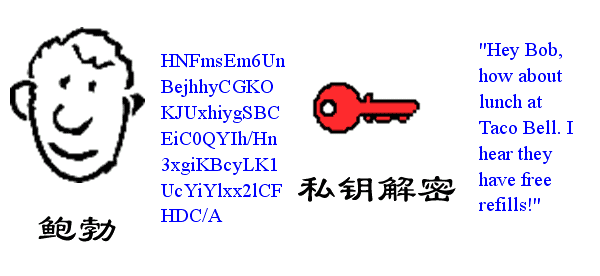
\includegraphics[width=8cm]{bg4}
    \end{figure}
    鲍勃收信后,用私钥解密,就看到了信件内容。这里要强调的是,只要鲍勃的私钥不泄露,这封信就是安全的,即使落在别人手里,也无法解密。
  \end{center}
\end{frame}

\begin{frame}
  \transboxout
  \frametitle{RSA加密算法}
  \begin{center}
    \begin{figure}
      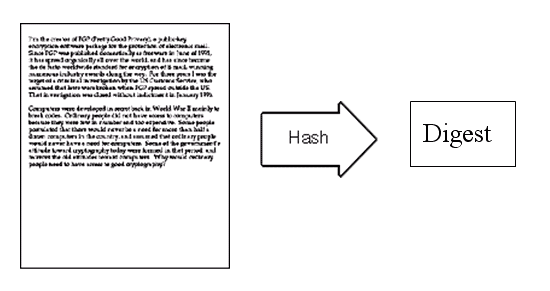
\includegraphics[width=8cm]{bg5}
    \end{figure}
    鲍勃给苏珊回信,决定采用"数字签名"。他写完后先用Hash函数,生成信件的摘要(digest)。
  \end{center}
\end{frame}

\begin{frame}
  \transboxout
  \frametitle{RSA加密算法}
  \begin{center}
    \begin{figure}
      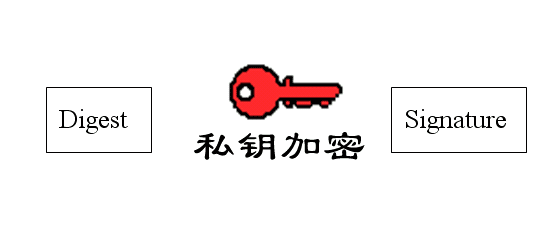
\includegraphics[width=8cm]{bg6}
    \end{figure}
    然后,鲍勃使用私钥,对这个摘要加密,生成"数字签名"(signature)。
  \end{center}
\end{frame}

\begin{frame}
  \transboxout
  \frametitle{RSA加密算法}
  \begin{center}
    \begin{figure}
      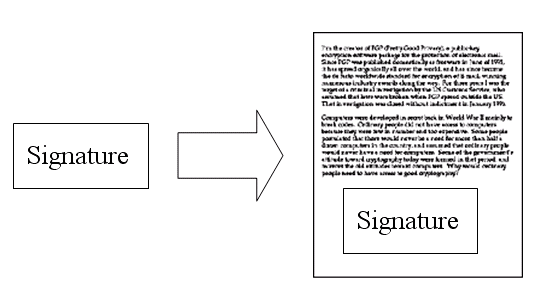
\includegraphics[width=8cm]{bg7}
    \end{figure}
    鲍勃将这个签名,附在信件下面,一起发给苏珊。
  \end{center}
\end{frame}

\begin{frame}
  \transboxout
  \frametitle{RSA加密算法}
  \begin{center}
    \begin{figure}
      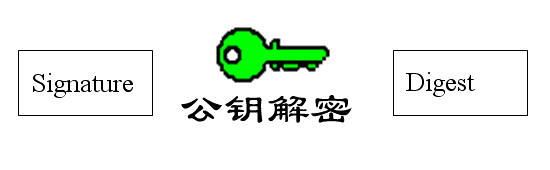
\includegraphics[width=8cm]{bg8}
    \end{figure}
    苏珊收信后,取下数字签名,用鲍勃的公钥解密,得到信件的摘要。由此证明,这封信确实是鲍勃发出的。
  \end{center}
\end{frame}

\begin{frame}
  \transboxout
  \frametitle{RSA加密算法}
  \begin{center}
    \begin{figure}
      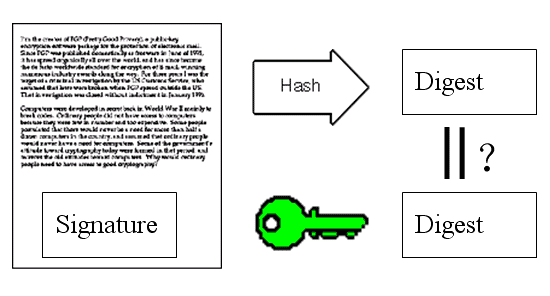
\includegraphics[width=8cm]{bg9}
    \end{figure}
    苏珊再对信件本身使用Hash函数,将得到的结果,与上一步得到的摘要进行对比。如果两者一致,就证明这封信未被修改过。
  \end{center}
\end{frame}

\begin{frame}
  \transboxout
  \frametitle{RSA加密算法}
  \begin{center}
    \begin{figure}
      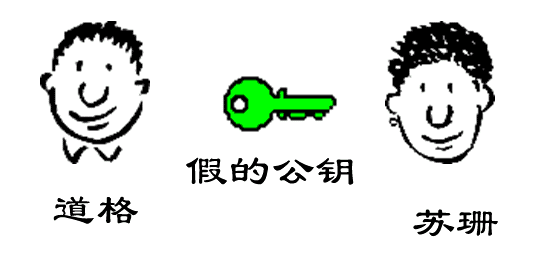
\includegraphics[width=8cm]{bg10}
    \end{figure}
    复杂的情况出现了。道格想欺骗苏珊,他偷偷使用了苏珊的电脑,用自己的公钥换走了鲍勃的公钥。此时,苏珊实际拥有的是道格的公钥,但是还以为这是鲍勃的公钥。因此,道格就可以冒充鲍勃,用自己的私钥做成"数字签名",写信给苏珊,让苏珊用假的鲍勃公钥进行解密。
  \end{center}
\end{frame}

\begin{frame}
  \transboxout
  \frametitle{RSA加密算法}
  \begin{center}
    \begin{figure}
      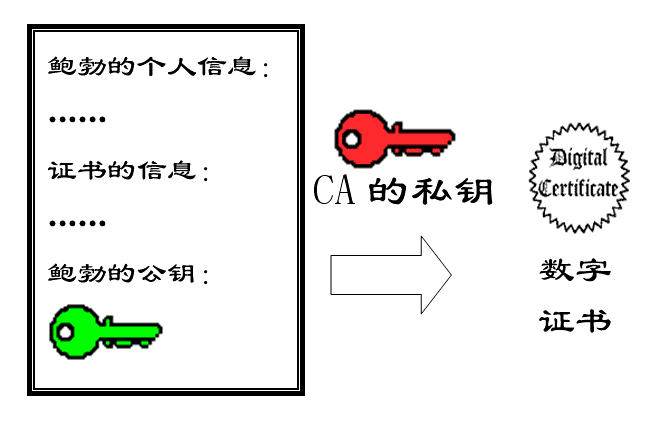
\includegraphics[width=7cm]{bg11}
    \end{figure}
    后来,苏珊感觉不对劲,发现自己无法确定公钥是否真的属于鲍勃。她想到了一个办法,要求鲍勃去找"证书中心"(certificate authority,简称CA),为公钥做认证。证书中心用自己的私钥,对鲍勃的公钥和一些相关信息一起加密,生成"数字证书"(Digital Certificate)。
  \end{center}
\end{frame}

\begin{frame}
  \transboxout
  \frametitle{RSA加密算法}
  \begin{center}
    \begin{figure}
      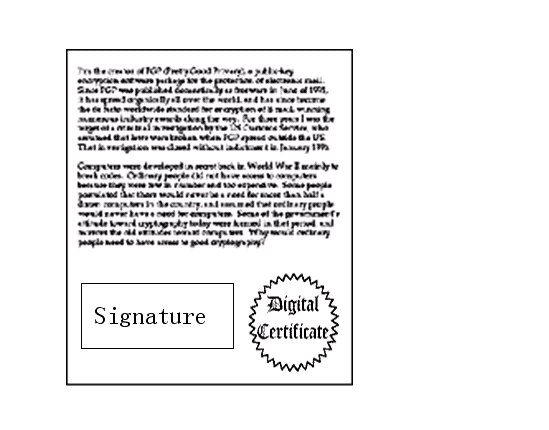
\includegraphics[width=7cm]{bg12}
    \end{figure}
    鲍勃拿到数字证书以后,就可以放心了。以后再给苏珊写信,只要在签名的同时,再附上数字证书就行了。
  \end{center}
\end{frame}

\begin{frame}
  \transboxout
  \frametitle{RSA加密算法}
  \begin{center}
    \begin{figure}
      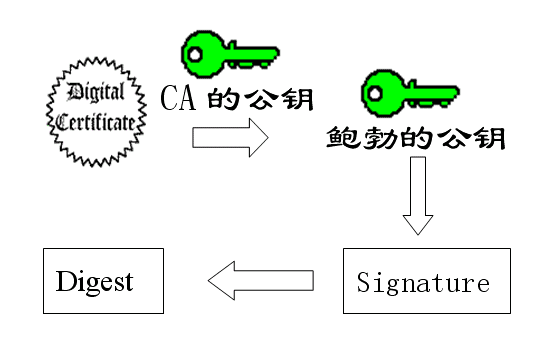
\includegraphics[width=8cm]{bg13}
    \end{figure}
    苏珊收信后,用CA的公钥解开数字证书,就可以拿到鲍勃真实的公钥了,然后就能证明"数字签名"是否真的是鲍勃签的。
  \end{center}
\end{frame}



%\begin{frame}
%  \transboxout
%  \frametitle{RSA加密算法}
%  \begin{center}
%    \begin{figure}
%      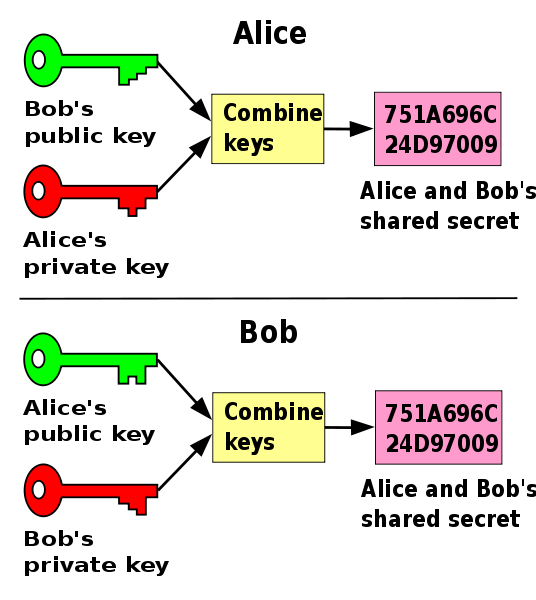
\includegraphics[width=6cm]{Publickeysharedsecret.svg.png}
%    \end{figure}
%  \end{center}
%\end{frame}

\section{获奖者生平}
% http://www.techcn.com.cn/index.php?doc-view-131079.html#1

\begin{frame}
  \transwipe
  \frametitle{获奖啦}
  \parpic(11cm,6cm){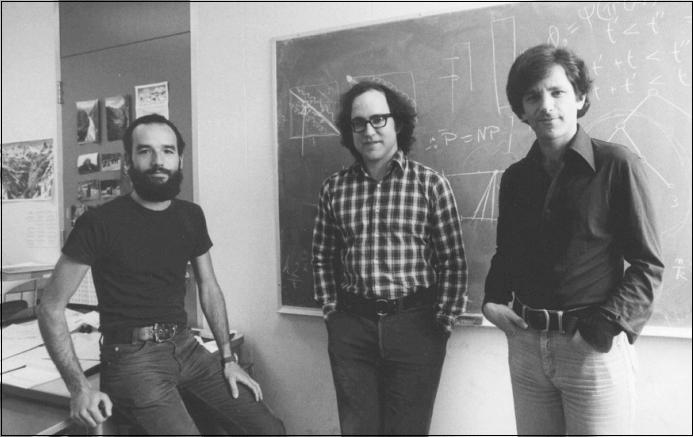
\includegraphics[width=9cm]{3peoples}}

\end{frame}

\begin{frame}
  \transboxout
  \frametitle{获奖啦}
  \parpic(11cm,6cm){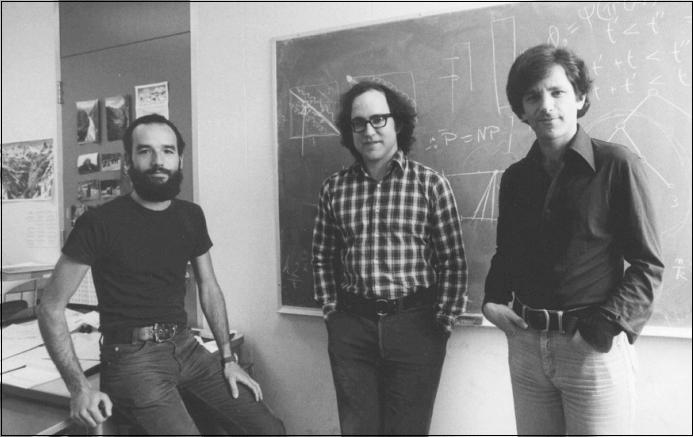
\includegraphics[width=9cm]{3peoples}}
  \parpic(11cm,6cm){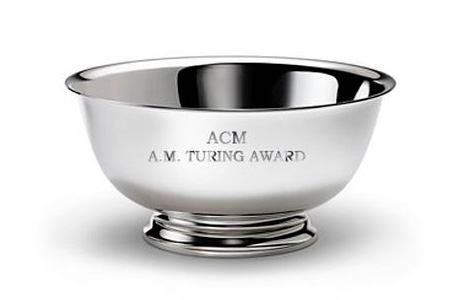
\includegraphics[width=5cm]{turing}}


\end{frame}

\subsection{\hfill Cocks}
\begin{frame}
  \frametitle{Clifford Cocks}
  
  \begin{multicols}{2}
    \begin{figure}
      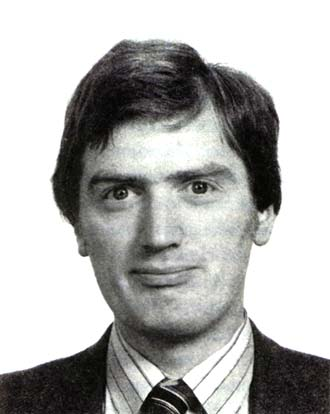
\includegraphics[width=3cm]{Cocks.jpg}
      \caption{1950,Prestbury, Cheshire, United Kingdom}
    \end{figure}
    \small

    He invented the widely used encryption algorithm now commonly known as RSA, about three years before it was independently developed by Rivest, Shamir, and Adleman at MIT. He has not been generally recognised for this achievement because his work was classified information, and therefore not released to the public at the time.

    
  \end{multicols}
  
\end{frame}

\subsection{\hfill Rivest}
\begin{frame}
  \frametitle{Ronald L. Rivest}
  \begin{multicols}{2}
    \begin{figure}
      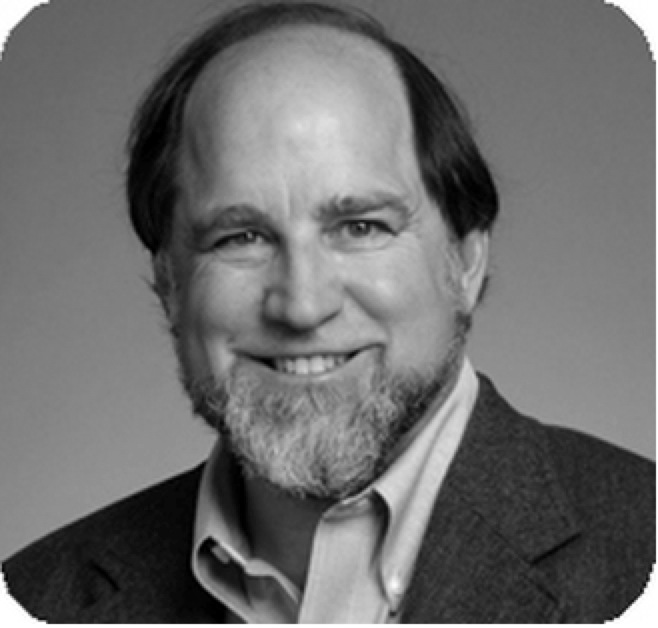
\includegraphics[width=3cm]{r.png}
      \caption{1947, Schenectady, New York, USA}
    \end{figure}

\footnotesize

   BA (Mathematics, Yale University, 1969);

    ~\\

   PhD (Computer Science, Standford University, 1973); 

    ~\\

   Robert W Floyd. 1978. 

    ~\\

   Donald Ervin Knuth. 1974. 

    ~\\

   Postdoctoral (Computer Science, INRIA, 1975);
   
   ~\\
   
   RSA Algorithm 1977

    ~\\

   RSA Data Security  1983

    ~\\

   Introduction to Algorithms 1990

    
  \end{multicols}
  
\end{frame}


\subsection{\hfill Shamir}

% EDUCATION
\begin{frame}
  \frametitle{Adi Shamir}
  \begin{multicols}{2}
    \begin{minipage}[c]{0.5\textwidth}
      \begin{figure}[H]
        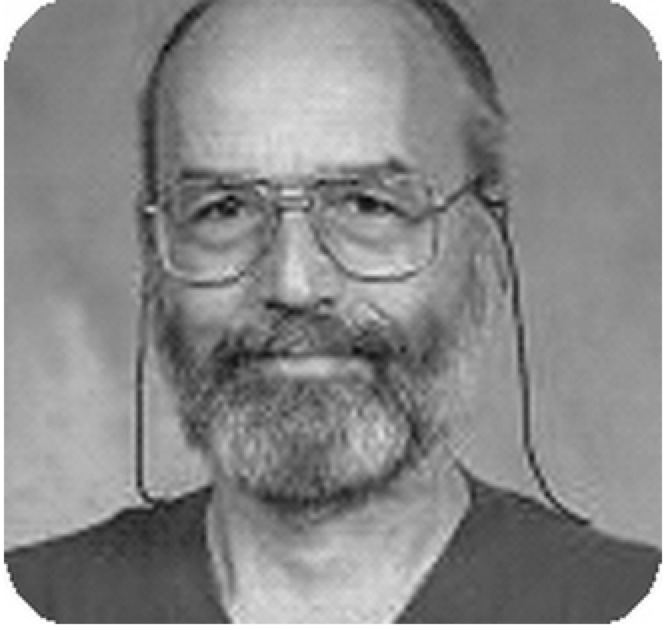
\includegraphics[width=3cm]{s.png}
        \caption{July 6, 1952, Tel Aviv, Israel}
      \end{figure}
    \end{minipage}
\footnotesize
    BSc (Mathematics, Tel Aviv University, 1973); 
   
    ~\\

    MSc (Computer Science, Weizmann Institute, Israel, 1975); 
    
    ~\\

    PhD (Computer Science, Weizmann Institute, Israel, 1977)    

    ~\\

    Shamir's Secret Sharing.

    ~\\

    Attack DES, 1977

    ~\\

    Identity-based crtyptography, 1984

    ~\\

    Visual cryptography, 1994

  \end{multicols}
  
\end{frame}
% HONORS & AWARDS

\subsection{\hfill Adleman}
\begin{frame}
  \frametitle{Leonard M. Adleman}
  \begin{multicols}{2}
    \begin{figure}
      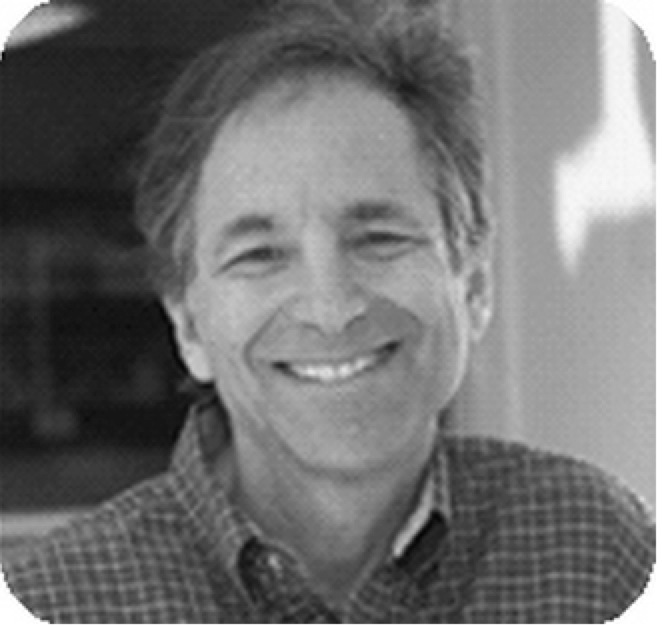
\includegraphics[width=3cm]{a.png}
      \caption{December 31, 1945, San Francisco, USA}
    \end{figure}
\footnotesize
    BA, Mathematics (University of California, Berkley, 1968);

    ~\\

    PhD, Computer Science (University of California, Berkley, 1976).

    ~\\

    Professor (University of Southern California, 1980).

    ~\\

    Godfather Of Computer Virus, Student Cohen. 1983.

    ~\\

    Father of DNA Computing. 

    ~\\

    Fermat's Last Theorem 1986.

    ~\\

    Hollywood Film Sneakers, mathmatical and cryptography consultant 1992 
    
  \end{multicols}

\end{frame}

\section{八卦环节}
\begin{frame}
  \transblindsvertical
  \frametitle{八卦环节}
 ~~~~当年第一个公开密钥算法是背包算法,其发明者Ralph Merkle对这个算法极有信心,确信这个算法不可能被攻破,所以他悬赏100美元奖金给破解算法的人。Adi Shamir迅速破解了该算法,并领走了奖金。Shamir就是RSA算法的发明人之一。

 ~~~~但Merkle并没有气馁,他又加强了算法,并悬赏1000美元奖金,给破解新算法的人。结果Ronald Rivest也迅速地破解了该算法,并领走了奖金。Rivest是RSA算法的另一个发明人。

 ~~~~于是,Merkle终于没有胆量尝试第三次悬赏,于是RSA的最后一个作者Leonard Adleman也就没有机会成为万元户了。(按照规律,Merkle如果要悬赏,应该是10000美金了。)
\end{frame}









%\begin{frame}
%\frametitle{我是中文} 
%%\framesubtitle{\centerline{subtext}} 
%\animate<3-6>% 自动逐步显示
%\begin{itemize}[<+->]
%\item one
%\item two
%\item three
%\item four
%\item five
%\item six
%\end{itemize}
%
%刘正 徐小奇 e
%\end{frame}



















\end{document}
